\chapter{Составные бозоны, спиновые представления и удвоение Дирака}

\section{Обменная симметрия и составные бозоны}

Начальный вопрос — это подлинный парадокс о составных частицах. Если два фермиона образуют бозон, могут ли два таких бозона занимать одно и то же состояние, не нарушая фермионного запрета? Ответ начинается с самого правила обмена.

Пусть две тождественные частицы описываются волновой функцией двух аргументов. Символы \(x\) и \(y\) помечают два места, соответствующие двум частицам; они не различают два вида частиц. Для бозонов волновая функция симметрична, а для фермионов антисимметрична:
\begin{equation}
\Psi_B(x,y)=\Psi_B(y,x),
\qquad
\Psi_F(x,y)=-\Psi_F(y,x).
\end{equation}
Эта симметрия означает, что перестановка двух неразличимых частиц не создаёт нового физического состояния.

Два бозона, конечно, могут занимать одно и то же одночастичное состояние. Если это состояние имеет волновую функцию \(\varphi\), то двухчастичное произведение равно
\begin{equation}
\Psi(x,y)=\varphi(x)\varphi(y).
\end{equation}
Волновые функции — это обычные комплекснозначные функции, а не операторы и не матрицы, поэтому их значения коммутируют:
\begin{equation}
\varphi(x)\varphi(y)=\varphi(y)\varphi(x).
\end{equation}
Следовательно, произведение симметрично. Та же конструкция не может дать ненулевое двухфермионное состояние, поскольку антисимметрия потребовала бы
\begin{equation}
\varphi(x)\varphi(y)=-\varphi(y)\varphi(x),
\end{equation}
тогда как обе стороны без знака минус равны.

В более общем случае начнём с любой двухчастичной волновой функции \(F(x,y)\), не предполагая никакой обменной симметрии. Её симметрическая и антисимметрическая части с точностью до нормировки имеют вид
\begin{align}
F_{\mathrm{sym}}(x,y)&=F(x,y)+F(y,x),\\
F_{\mathrm{asym}}(x,y)&=F(x,y)-F(y,x).
\end{align}
Проверка на обмен записывается явно:
\begin{align}
F_{\mathrm{sym}}(y,x)
&=F(y,x)+F(x,y)
=F_{\mathrm{sym}}(x,y),\\
F_{\mathrm{asym}}(y,x)
&=F(y,x)-F(x,y)
=-F_{\mathrm{asym}}(x,y).
\end{align}
Прибавление функции с переставленными аргументами симметризует её; вычитание функции с переставленными аргументами антисимметризует её.

Пара атомов водорода даёт более интересный случай. Здесь есть четыре фермиона-составляющих: два тождественных электрона и два тождественных протона. Пусть \(x_1,x_2\) обозначают электронные переменные, а \(y_1,y_2\) — протонные. Четырёхчастичная волновая функция должна быть отдельно антисимметрична при обмене электронов и при обмене протонов:
\begin{align}
\Psi(x_2,x_1;y_1,y_2)
&=-\Psi(x_1,x_2;y_1,y_2),\\
\Psi(x_1,x_2;y_2,y_1)
&=-\Psi(x_1,x_2;y_1,y_2).
\end{align}

Чтобы ввести две различные одноатомные волновые функции, представим один атом водорода, локализованный вблизи начала координат, с волновой функцией \(\psi(x,y)\), и другой, локализованный в другом месте, с волновой функцией \(\phi(x,y)\). Вторая может быть просто сдвинутой копией первой, полученной переносом обоих её аргументов, электронного и протонного, но в этой постановке она всё равно является другой волновой функцией. Наивное произведение имеет вид
\begin{equation}
\psi(x_1,y_1)\phi(x_2,y_2).
\end{equation}
Оно пока не обладает ни одной из требуемых фермионных антисимметрий.

Сначала антисимметризуем по электронным переменным:
\begin{equation}
\Psi_x=
\psi(x_1,y_1)\phi(x_2,y_2)
-\psi(x_2,y_1)\phi(x_1,y_2).
\end{equation}
При \(x_1\leftrightarrow x_2\) два члена меняются местами, и всё выражение меняет знак. Теперь антисимметризуем этот результат по протонным переменным. Порядок четырёх членов фиксируется двумя последовательными антисимметризациями.\footnote{Эта конструкция также фиксирует схему знаков \(+,-,-,+\) благодаря исправлениям меток переменных, сделанным в устном вычислении.}
\begin{align}
\Psi_{2H}(x_1,x_2;y_1,y_2)
&=\Psi_x(x_1,x_2;y_1,y_2)\nonumber\\
&\quad{}-\Psi_x(x_1,x_2;y_2,y_1)\\
&=\psi(x_1,y_1)\phi(x_2,y_2)\nonumber\\
&\quad{}-\psi(x_2,y_1)\phi(x_1,y_2)\nonumber\\
&\quad{}-\psi(x_1,y_2)\phi(x_2,y_1)\nonumber\\
&\quad{}+\psi(x_2,y_2)\phi(x_1,y_1).
\label{eq:two-hydrogen-antisymmetrized}
\end{align}
Обмен электронов переставляет местами первые два члена и последние два члена с общим изменением знака. То же делает и обмен протонов. Следовательно, состояние обладает в точности двумя отдельными антисимметриями, требуемыми для фермионов-составляющих.

\begin{classroomqa}
\lecturetimestamp{00:11:11}
\audiencequestion{Если атомы водорода — бозоны, то что мешает поместить два из них прямо друг на друга?}
\lecturerresponse{Бозонная обменная статистика не устраняет силы между атомами. Запрет Паули для составляющих вместе с другими межатомными силами может сделать пространственное перекрытие чрезвычайно энергетически затратным. Это не то же самое, что спрашивать, могут ли атомы занимать одно и то же делокализованное состояние с определённым импульсом. Собственное состояние импульса распределено по всему пространству, так что общий импульс не означает вталкивания атомов в одну и ту же точку. Даже объекты с жёстким ядром, такие как бильярдные шары, могли бы подчиняться бозонной обменной статистике: их жёсткие ядра препятствовали бы пространственному перекрытию, а бозонная статистика всё равно допускала бы занятие одного и того же импульсного состояния.}
\end{classroomqa}

\begin{classroomqa}
\lecturetimestamp{00:12:28}
\audiencequestion{Если поместить два атома водорода в одно и то же собственное состояние импульса, окажутся ли их составляющие фермионы в одном и том же состоянии?}
\lecturerresponse{Нет. Четырёхчастичное состояние остаётся антисимметричным при обмене двух электронных переменных и отдельно антисимметричным при обмене двух протонных переменных. Симметричен только одновременный обмен обеих составляющих---то есть обмен двух атомов как целых---.}
\end{classroomqa}

В самом деле, обмен двух атомов означает выполнение обеих подстановок
\begin{equation}
x_1\leftrightarrow x_2,
\qquad
y_1\leftrightarrow y_2.
\end{equation}
Первая подстановка даёт один фермионный знак минус, и вторая даёт ещё один:
\begin{equation}
\begin{aligned}
\Psi_{2H}(x_2,x_1;y_2,y_1)
&=(-1)(-1)\Psi_{2H}(x_1,x_2;y_1,y_2)\\
&=\Psi_{2H}(x_1,x_2;y_1,y_2).
\end{aligned}
\end{equation}
То же видно и почленно в уравнении~\eqref{eq:two-hydrogen-antisymmetrized}. При обмене целых атомов
\begin{equation}
\psi(x_1,y_1)\phi(x_2,y_2)
\longleftrightarrow
\psi(x_2,y_2)\phi(x_1,y_1),
\end{equation}
поэтому первый и четвёртый члены переставляются местами. Аналогично,
\begin{equation}
-\psi(x_2,y_1)\phi(x_1,y_2)
\longleftrightarrow
-\psi(x_1,y_2)\phi(x_2,y_1),
\end{equation}
поэтому второй и третий члены переставляются местами. Полное состояние симметрично относительно перестановки атомов. Два минуса от составляющих дают составному объекту плюс.

Это утверждение об обмене логически независимо от энергии, необходимой для перекрытия атомов. Сильное отталкивание может сделать такое перекрытие недоступным, но оно не меняет симметричный закон обмена.

\begin{classroomqa}
\lecturetimestamp{00:14:42}
\audiencequestion{Что физически представляет собой построенное четырёхчастичное состояние, и является ли оно именно состоянием в импульсном пространстве?}
\lecturerresponse{Это двухатомная волновая функция, полученная из двух одноатомных волновых функций антисимметризацией сначала по электронным меткам, а затем по протонным. Её не обязательно записывать в импульсном представлении. Переменные могут относиться к координатному, импульсному или иному представлению; требуемые симметрии обмена составляющих остаются теми же.}
\end{classroomqa}

Следовательно, два атома могут занимать одну и ту же делокализованную импульсную волновую функцию, хотя принудительное сильное перекрытие их пространственных распределений может требовать очень большой энергии.

Теперь положим две одноатомные волновые функции равными, \(\phi=\psi\). Тогда уравнение~\eqref{eq:two-hydrogen-antisymmetrized} принимает вид
\begin{align}
\Psi_{\mathrm{same}}
&=\psi(x_1,y_1)\psi(x_2,y_2)
-\psi(x_2,y_1)\psi(x_1,y_2)\nonumber\\
&\quad
-\psi(x_1,y_2)\psi(x_2,y_1)
+\psi(x_2,y_2)\psi(x_1,y_1).
\end{align}

Обращается ли это четырёхчастичное состояние в нуль? Нет. Первое и четвёртое произведения равны, и второе и третье произведения равны. Используя коммутативность одноатомных волновых функций,
\begin{equation}
\Psi_{\mathrm{same}}
=
2\left[
\psi(x_1,y_1)\psi(x_2,y_2)
-\psi(x_2,y_1)\psi(x_1,y_2)
\right],
\label{eq:same-hydrogen-state}
\end{equation}
что, вообще говоря, не равно нулю. Оно остаётся антисимметричным по двум электронным переменным и отдельно антисимметричным по двум протонным переменным.

Здесь нет приписывания по одному точно локализованному электрону каждому точно локализованному атому. Электрон, связанный в атоме, пространственно делокализован в пределах своей атомной волновой функции. Поэтому придание двум атомам одного и того же атомного состояния не означает ни \(x_1=x_2\), ни \(y_1=y_2\).

Запрет для составляющих проявляется при прямой проверке совпадения аргументов. Если два моделируемых электронных аргумента совпадают, \(x_1=x_2=x\), то уравнение~\eqref{eq:same-hydrogen-state} даёт
\begin{align}
\Psi_{\mathrm{same}}(x,x;y_1,y_2)
&=2\bigl[
\psi(x,y_1)\psi(x,y_2)\nonumber\\
&\quad{}-\psi(x,y_1)\psi(x,y_2)
\bigr]\\
&=0.
\end{align}
Соответствующее выражение также обращается в нуль при \(y_1=y_2\). Таким образом, составная волновая функция для одинакового состояния не равна нулю, тогда как её амплитуда при совпадающих аргументах тождественных фермионов обращается в нуль.\footnote{В этой модели спин и любые другие одночастичные метки опущены. Фермионная антисимметрия относится к полному набору одночастичных меток; показанное сокращение касается совпадения тех аргументов, которые здесь сохранены.}

\begin{classroomqa}
\lecturetimestamp{00:20:41}
\audiencequestion{Могут ли атомы находиться в одном и том же состоянии, тогда как их электроны и протоны не находятся в одних и тех же состояниях составляющих?}
\lecturerresponse{Да. Равенство составных атомных волновых функций не устраняет отдельные электронную и протонную антисимметрии. Полное четырёхчастичное состояние может описывать два атома в одном атомном состоянии, приписывая при этом нулевую амплитуду совпадающим аргументам тождественных фермионов.}
\end{classroomqa}

\begin{classroomqa}
\lecturetimestamp{00:21:12}
\audiencequestion{Исключила ли антисимметризация те компоненты, в которых совпадают тождественные составляющие?}
\lecturerresponse{Да. В показанных здесь переменных такие компоненты точно взаимно уничтожаются. Точное утверждение таково: антисимметричная волновая функция обращается в нуль, когда два аргумента тождественных фермионов равны.}
\end{classroomqa}

Это сокращение не зависело от предварительного приравнивания атомных волновых функций. Для общего состояния в уравнении~\eqref{eq:two-hydrogen-antisymmetrized},
\begin{align}
\Psi_{2H}(x,x;y_1,y_2)
&=\psi(x,y_1)\phi(x,y_2)\nonumber\\
&\quad{}-\psi(x,y_1)\phi(x,y_2)\nonumber\\
&\quad{}-\psi(x,y_2)\phi(x,y_1)\nonumber\\
&\quad{}+\psi(x,y_2)\phi(x,y_1)\\
&=0.
\end{align}

\begin{classroomqa}
\lecturetimestamp{00:21:32}
\audiencequestion{Сохраняется ли это сокращение, когда атомы находятся в разных состояниях и переменные тождественных составляющих совпадают?}
\lecturerresponse{Да. Оно следует из самой антисимметрии, а не из условия \(\phi=\psi\). То же утверждение верно и в другом представлении: после перехода в импульсное пространство амплитуда обращается в нуль, когда совпадают два импульсных аргумента тождественных фермионов, при условии что совпадают и другие опущенные одночастичные метки.}
\end{classroomqa}

\section{Спин как конечномерная квантовая система}

Математика спина вновь возникает при рассмотрении изоспина, цвета и других внутренних симметрий физики элементарных частиц. Аналогия здесь формальная: появляется одна и та же алгебра, хотя физические величины не обязаны иметь одну и ту же интерпретацию. Ближайшая задача — продвинуться в изучении спина ещё немного, а затем вернуться к уравнению Дирака. Позже этот аппарат будет использован для изоспина — понятия, исторически связанного с 1930-ми годами.

Электрон — частица со спином \(\tfrac12\); то же верно для протона и мюона. \(z\)-компонента его спина может принимать два значения. Прежде чем фиксировать единицы, запишем
\begin{equation}
S_z=m\hbar.
\end{equation}
Отныне \(\hbar=1\). Букву \(L\) по соглашению оставляют для орбитального момента импульса, поэтому собственный спин будем обозначать через \(S\). Для него выполняется та же алгебра момента импульса:
\begin{equation}
[S_x,S_y]=iS_z,
\quad
[S_y,S_z]=iS_x,
\quad
[S_z,S_x]=iS_y,
\end{equation}
и
\begin{equation}
S_\pm=S_x\pm iS_y.
\end{equation}
Оператор \(S_+\) повышает собственное значение \(S_z\), а \(S_-\) понижает его.

\begin{classroomqa}
\lecturetimestamp{00:25:39}
\audiencequestion{Речь идёт именно о собственном спине?}
\lecturerresponse{Да, здесь имеется в виду именно собственный спин. Та же алгебра момента импульса применима и в более общем случае, в том числе к орбитальному моменту импульса или к вращению макроскопического тела.}
\end{classroomqa}

Для спина 1/2 единственные собственные значения \(S_z\) равны \(+\tfrac12\) и \(-\tfrac12\). Пока отвлечёмся от всего остального, что относится к электрону: забудем о его положении и импульсе и сохраним только два спиновых состояния. Тогда
\begin{equation}
|\psi\rangle
=
\alpha|\uparrow_z\rangle+\beta|\downarrow_z\rangle
\quad\longleftrightarrow\quad
\begin{pmatrix}
\alpha\\
\beta
\end{pmatrix},
\end{equation}
где
\begin{equation}
|\alpha|^2=P(\uparrow_z),
\qquad
|\beta|^2=P(\downarrow_z),
\qquad
|\alpha|^2+|\beta|^2=1.
\end{equation}
Это двумерное пространство состояний. Это не утверждение, что обычное пространство двумерно.

\begin{classroomqa}
\lecturetimestamp{00:28:18}
\audiencequestion{Было сказано, что физическое пространство двумерно?}
\lecturerresponse{Нет. Двумерно пространство спиновых состояний. Положение и импульс временно опущены, как если бы электрон был пригвождён к стене и можно было бы измерять только его спин.}
\end{classroomqa}

Операторы в этом пространстве состояний представляются матрицами \(2\times2\). Удобно выбрать базис \(S_z\) так, чтобы \(S_z\) был диагонален, но диагональный вид — это выбор базиса, а не физическое требование.

\begin{classroomqa}
\lecturetimestamp{00:29:46}
\audiencequestion{Должен ли \(S_z\) быть диагональным?}
\lecturerresponse{Нет. Его выбирают диагональным для удобства. Другие матричные представления физически эквивалентны.}
\end{classroomqa}

\begin{classroomqa}
\lecturetimestamp{00:30:08}
\audiencequestion{Является ли \(S_z\) матрицей?}
\lecturerresponse{\(S_z\) — наблюдаемая величина, а значит, оператор. В выбранном конечномерном базисе этот оператор представляется матрицей, действующей на векторы состояния.}
\end{classroomqa}

Особенно полезно представление
\begin{equation}
S_i=\frac12\sigma_i,
\end{equation}
где
\begin{equation}
\sigma_x=
\begin{pmatrix}
0&1\\
1&0
\end{pmatrix},
\quad
\sigma_y=
\begin{pmatrix}
0&-i\\
i&0
\end{pmatrix},
\quad
\sigma_z=
\begin{pmatrix}
1&0\\
0&-1
\end{pmatrix}.
\end{equation}
Матрицы без множителя одна вторая — это матрицы Паули; сами операторы спина содержат этот множитель. Непосредственное перемножение матриц подтверждает коммутационные соотношения. Представление не единственно: поворот осей или замена базиса дают другую эквивалентную тройку.

Это двухкомпонентное представление момента импульса для спина 1/2.

\subsection{Собственные состояния вдоль координатных осей}

Полезно решать уравнения на собственные значения покомпонентно. Поскольку собственные значения \(\sigma_i\) равны \(\pm1\), собственные значения \(S_i=\sigma_i/2\) равны \(\pm\tfrac12\).

Для \(\sigma_z\) два уравнения имеют вид
\begin{align}
\begin{pmatrix}
1&0\\
0&-1
\end{pmatrix}
\begin{pmatrix}
\alpha\\
\beta
\end{pmatrix}
&=
\begin{pmatrix}
\alpha\\
\beta
\end{pmatrix},
&
\begin{pmatrix}
1&0\\
0&-1
\end{pmatrix}
\begin{pmatrix}
\alpha\\
\beta
\end{pmatrix}
&=
-
\begin{pmatrix}
\alpha\\
\beta
\end{pmatrix}.
\end{align}

\begin{figure}[t]
\centering
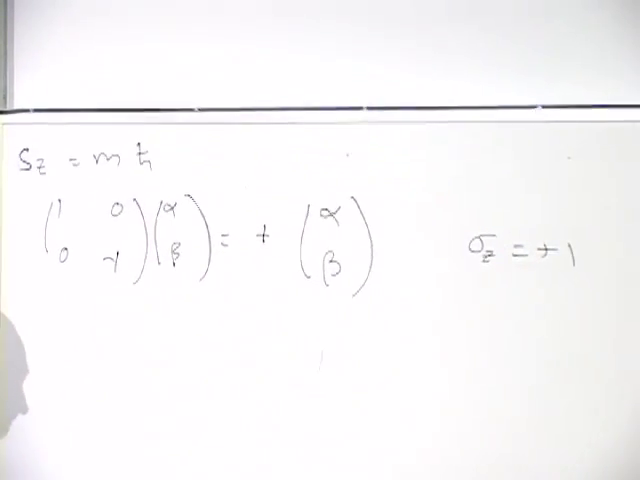
\includegraphics[width=0.74\textwidth]{lecture_08_figure_02.png}
\caption{Уравнение на собственное значение \(+1\) для \(\sigma_z\), действующей на двухкомпонентный спинор.}
\lectureframe{00:34:57}
\end{figure}

Для собственного значения \(+1\) построчное умножение даёт
\begin{equation}
\begin{pmatrix}
1\cdot\alpha+0\cdot\beta\\
0\cdot\alpha-\beta
\end{pmatrix}
=
\begin{pmatrix}
\alpha\\
-\beta
\end{pmatrix}
=
\begin{pmatrix}
\alpha\\
\beta
\end{pmatrix}.
\end{equation}
Верхнее уравнение выполняется автоматически, а нижнее даёт \(-\beta=\beta\), следовательно, \(\beta=0\). Нормировка требует \(|\alpha|=1\); выбирая несущественную общую фазу так, чтобы \(\alpha=1\),
\begin{equation}
|+z\rangle=
\begin{pmatrix}
1\\
0
\end{pmatrix}.
\end{equation}

Для собственного значения \(-1\),
\begin{equation}
\begin{pmatrix}
\alpha\\
-\beta
\end{pmatrix}
=
\begin{pmatrix}
-\alpha\\
-\beta
\end{pmatrix}.
\end{equation}
Теперь нижнее уравнение выполняется автоматически, а верхнее даёт \(\alpha=-\alpha\), поэтому \(\alpha=0\). Выбирая \(\beta=1\), получаем
\begin{equation}
|-z\rangle=
\begin{pmatrix}
0\\
1
\end{pmatrix}.
\end{equation}

Теперь изменим эксперимент и измерим \(S_x\). Поскольку
\begin{equation}
\sigma_x
\begin{pmatrix}
\alpha\\
\beta
\end{pmatrix}
=
\begin{pmatrix}
0\cdot\alpha+\beta\\
\alpha+0\cdot\beta
\end{pmatrix}
=
\begin{pmatrix}
\beta\\
\alpha
\end{pmatrix},
\end{equation}
уравнение для собственного значения \(+1\) принимает вид
\begin{equation}
\begin{pmatrix}
\beta\\
\alpha
\end{pmatrix}
=
\begin{pmatrix}
\alpha\\
\beta
\end{pmatrix}.
\end{equation}
Два покомпонентных уравнения, \(\beta=\alpha\) и \(\alpha=\beta\), выражают одно и то же условие. Из нормировки следует
\begin{equation}
2|\alpha|^2=1,
\end{equation}
поэтому удобно выбрать
\begin{equation}
|+x\rangle
=
\frac{1}{\sqrt2}
\begin{pmatrix}
1\\
1
\end{pmatrix}.
\end{equation}

\begin{figure}[t]
\centering
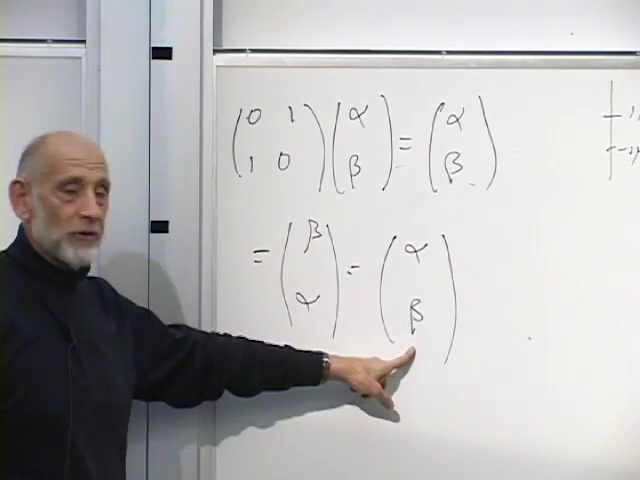
\includegraphics[width=0.74\textwidth]{lecture_08_figure_03.png}
\caption{Для собственного значения \(+1\) матрица \(\sigma_x\) переставляет две компоненты местами, что требует \(\alpha=\beta\).}
\lectureframe{00:39:42}
\end{figure}

\begin{classroomqa}
\lecturetimestamp{00:40:13}
\audiencequestion{Если бы множитель одна вторая был включён, было бы собственное значение равно одной второй?}
\lecturerresponse{Да. Матрица Паули \(\sigma_x\) имеет собственные значения \(\pm1\), тогда как \(S_x=\sigma_x/2\) имеет собственные значения \(\pm\tfrac12\).}
\end{classroomqa}

Для собственного значения \(-1\),
\begin{equation}
\begin{pmatrix}
\beta\\
\alpha
\end{pmatrix}
=
-
\begin{pmatrix}
\alpha\\
\beta
\end{pmatrix},
\end{equation}
поэтому
\begin{equation}
\beta=-\alpha,
\qquad
\alpha=-\beta.
\end{equation}
Это снова одно и то же уравнение. После нормировки
\begin{equation}
|-x\rangle
=
\frac{1}{\sqrt2}
\begin{pmatrix}
1\\
-1
\end{pmatrix}.
\end{equation}
Таким образом, равная суперпозиция состояний \(z\)-вверх и \(z\)-вниз поляризована вдоль положительной оси \(x\), тогда как та же суперпозиция с относительным знаком минус поляризована вдоль отрицательной оси \(x\).

Для направления \(y\),
\begin{equation}
\sigma_y
\begin{pmatrix}
\alpha\\
\beta
\end{pmatrix}
=
\begin{pmatrix}
-i\beta\\
i\alpha
\end{pmatrix}.
\end{equation}
Два нормированных собственных вектора имеют вид
\begin{equation}
|+y\rangle
=
\frac{1}{\sqrt2}
\begin{pmatrix}
1\\
i
\end{pmatrix},
\qquad
|-y\rangle
=
\frac{1}{\sqrt2}
\begin{pmatrix}
1\\
-i
\end{pmatrix},
\end{equation}
с точностью до общей фазы. Оба состояния дают вероятность \(1/2\) для \(z\)-вверх и \(1/2\) для \(z\)-вниз. Относительная фаза \(i\), которая не видна в этих двух вероятностях, отличает поляризацию по \(y\) от поляризации по \(x\). Линейные комбинации описывают также спин, поляризованный вдоль произвольных направлений; это вычисление пока откладывается.

\begin{classroomqa}
\lecturetimestamp{00:44:22}
\audiencequestion{Не приписан ли знак при \(i\) неверному собственному значению \(\sigma_y\)?}
\lecturerresponse{Знак и в самом деле мог быть приписан неправильному собственному значению. Здесь это соответствие не вполне определено; оно не устанавливается по памяти.}
\end{classroomqa}

Непосредственная проверка такова:
\begin{align}
\sigma_y\frac{1}{\sqrt2}
\begin{pmatrix}
1\\
i
\end{pmatrix}
&=
\frac{1}{\sqrt2}
\begin{pmatrix}
-i\,i\\
i
\end{pmatrix}
=
\frac{1}{\sqrt2}
\begin{pmatrix}
1\\
i
\end{pmatrix},\\
\sigma_y\frac{1}{\sqrt2}
\begin{pmatrix}
1\\
-i
\end{pmatrix}
&=
\frac{1}{\sqrt2}
\begin{pmatrix}
(-i)(-i)\\
i
\end{pmatrix}
=
-\frac{1}{\sqrt2}
\begin{pmatrix}
1\\
-i
\end{pmatrix}.
\end{align}
Следовательно, \(+i\) соответствует собственному значению \(+1\), а \(-i\) — собственному значению \(-1\).\footnote{После нескольких перемен в устном приписывании это соответствие так и остаётся неустоявшимся; приведённые здесь знаки фиксируются показанным умножением матриц.} Каждое состояние спина 1/2, в том числе любое состояние, поляризованное вдоль произвольного направления, является линейной комбинацией \(|+z\rangle\) и \(|-z\rangle\).

\section{Спин 1 и спиноры, зависящие от положения}

Для спина \(1\) возможные значения \(S_z\) равны \(+1,0,-1\). Поэтому пространство состояний трёхмерно. Спин \(1\) является целым спином и соответствует бозонной статистике. Мы ищем три матрицы \(3\times3\), удовлетворяющие тем же коммутационным соотношениям для момента импульса.

Ниже приведено представление, симметричное относительно трёх координатных направлений.\footnote{Знак \(S_y\) следует из матрицы, видимой около \(00{:}48{:}50\), и также фиксируется соотношением \([S_x,S_y]=iS_z\). Если изменить этот знак на противоположный, требуемый коммутатор изменил бы знак.}
\begin{equation}
\begin{aligned}
S_x
&=
i
\begin{pmatrix}
0&0&0\\
0&0&1\\
0&-1&0
\end{pmatrix},
&
S_y
&=
i
\begin{pmatrix}
0&0&1\\
0&0&0\\
-1&0&0
\end{pmatrix},\\
S_z
&=
i
\begin{pmatrix}
0&1&0\\
-1&0&0\\
0&0&0
\end{pmatrix}.
\end{aligned}
\end{equation}
Каждая матрица равна \(i\), умноженному на вещественную антисимметричную матрицу. В каждой есть одна \(1\), одна \(-1\) и нулевые строка и столбец, относящиеся к соответствующей координате: у \(S_x\) это первые, у \(S_y\) — вторые, а у \(S_z\) — третьи. Это даёт полезную мнемонику. В этом представлении \(S_z\) не диагонален.

Пусть
\begin{equation}
v=
\begin{pmatrix}
\alpha\\
\beta\\
\gamma
\end{pmatrix}.
\end{equation}
Тогда
\begin{equation}
S_zv
=
\begin{pmatrix}
i\beta\\
-i\alpha\\
0
\end{pmatrix}.
\end{equation}
Для собственного значения \(+1\),
\begin{equation}
i\beta=\alpha,
\qquad
-i\alpha=\beta,
\qquad
0=\gamma.
\end{equation}
Следовательно, \(\beta=-i\alpha\) и \(\gamma=0\). Из нормировки следует \(2|\alpha|^2=1\), поэтому
\begin{equation}
|m=+1\rangle
=
\frac{1}{\sqrt2}
\begin{pmatrix}
1\\
-i\\
0
\end{pmatrix}.
\end{equation}
Для собственного значения \(-1\),
\begin{equation}
i\beta=-\alpha,
\qquad
-i\alpha=-\beta,
\qquad
0=-\gamma,
\end{equation}
откуда \(\beta=i\alpha\), \(\gamma=0\) и
\begin{equation}
|m=-1\rangle
=
\frac{1}{\sqrt2}
\begin{pmatrix}
1\\
i\\
0
\end{pmatrix}.
\end{equation}
Наконец, уравнение для нулевого собственного значения даёт \(\alpha=\beta=0\), оставляя \(\gamma\) произвольным. Соответствующее нормированное решение имеет вид
\begin{equation}
|m=0\rangle
=
\begin{pmatrix}
0\\
0\\
1
\end{pmatrix}.
\end{equation}
Других собственных значений нет: этими тремя собственными векторами исчерпывается трёхмерное пространство. Множители \(1/\sqrt2\) не являются косметическими. Те же коэффициенты позднее войдут в количественные экспериментальные предсказания, когда эта алгебра будет применена к изоспину.

\begin{classroomqa}
\lecturetimestamp{00:54:10}
\audiencequestion{Как следует читать комплексные компоненты этих собственных векторов спина 1?}
\lecturerresponse{Для \(m=+1\) компоненты равны \(1/\sqrt2,-i/\sqrt2,0\); для \(m=-1\) — \(1/\sqrt2,i/\sqrt2,0\); а для \(m=0\) — \(0,0,1\).}
\end{classroomqa}

Другие тройки матриц удовлетворяют той же алгебре и физически эквивалентны. Приведённое выше симметричное представление полезно потому, что три направления в нём рассматриваются одинаково, и в дальнейшем оно ещё будет использоваться.

\subsection{Возвращение положения}

Теперь вернём движение частицы. Спин коммутирует с положением и с импульсом, так что любое из них можно задавать вместе с одной компонентой спина. Положение и импульс не коммутируют, и различные компоненты спина не коммутируют друг с другом.

Движущаяся частица со спином 1/2 описывается спинором, зависящим от положения,
\begin{equation}
\psi(x)=
\begin{pmatrix}
\psi_\uparrow(x)\\
\psi_\downarrow(x)
\end{pmatrix}.
\end{equation}
Величины
\begin{equation}
\rho_{\uparrow_z}(x)=|\psi_\uparrow(x)|^2,
\qquad
\rho_{\downarrow_z}(x)=|\psi_\downarrow(x)|^2
\end{equation}
являются совместными плотностями вероятности по положению и спину. Их сумма,
\begin{equation}
\rho(x)=\psi^\dagger(x)\psi(x)
=|\psi_\uparrow(x)|^2+|\psi_\downarrow(x)|^2,
\end{equation}
является плотностью вероятности по положению. Если известно, что частица была зарегистрирована в точке \(x\), то условные вероятности равны
\begin{equation}
P(\uparrow_z\mid x)
=
\frac{|\psi_\uparrow(x)|^2}{\psi^\dagger(x)\psi(x)},
\qquad
P(\downarrow_z\mid x)
=
\frac{|\psi_\downarrow(x)|^2}{\psi^\dagger(x)\psi(x)},
\end{equation}
всякий раз, когда \(\rho(x)\neq0\). Таким образом, электрон представляется двухкомпонентной пространственной волновой функцией, причём локальные амплитуды спина могут меняться от точки к точке.

Для движущейся частицы со спином 1 запишем
\begin{equation}
\phi(x)=
\begin{pmatrix}
\phi_1(x)\\
\phi_2(x)\\
\phi_3(x)
\end{pmatrix}.
\end{equation}
В каждой точке пространства три компоненты образуют вектор в том же спиновом пространстве, которое использовалось выше. Частицы со спином 1 имеют целый спин и являются бозонами.

\begin{classroomqa}
\lecturetimestamp{01:00:10}
\audiencequestion{Является ли \(\phi_1(x)\) само по себе вероятностью результата \(m=+1\) для частицы со спином 1?}
\lecturerresponse{Нет. Это амплитуда в выбранном трехкомпонентном базисе. Чтобы получить определенный спиновый исход, нужно взять бра соответствующего нормированного собственного вектора, спроецировать на него поле и взять квадрат модуля.}
\end{classroomqa}

\begin{figure}[t]
\centering
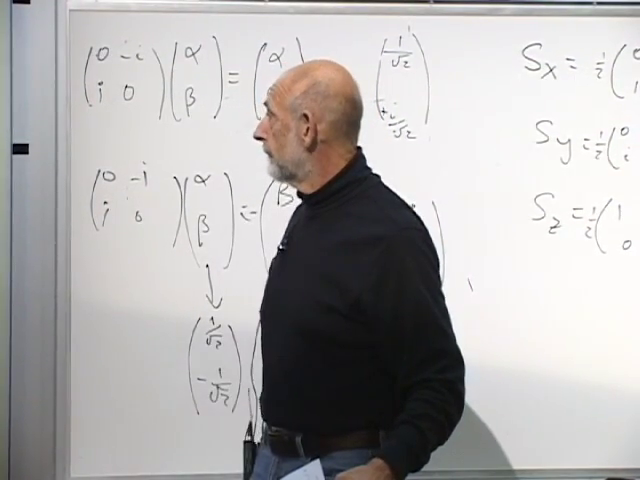
\includegraphics[width=0.82\textwidth]{lecture_08_figure_04.png}
\caption{Нормированные собственные векторы \(\sigma_y\) вместе с тремя матрицами для спина 1/2.}
\lectureframe{01:00:12}
\end{figure}

Например,
\begin{equation}
\begin{aligned}
|m=+1\rangle
&=
\frac{1}{\sqrt2}
\begin{pmatrix}
1\\
-i\\
0
\end{pmatrix}
\\
\Longrightarrow\quad\langle m=+1|
&=
\frac{1}{\sqrt2}
\begin{pmatrix}
1&i&0
\end{pmatrix}.
\end{aligned}
\end{equation}
Следовательно, амплитуда проекции равна
\begin{align}
\langle m=+1|\phi(x)\rangle
&=
\frac{1}{\sqrt2}
\begin{pmatrix}
1&i&0
\end{pmatrix}
\begin{pmatrix}
\phi_1(x)\\
\phi_2(x)\\
\phi_3(x)
\end{pmatrix}\\
&=
\frac{\phi_1(x)+i\phi_2(x)}{\sqrt2}.
\end{align}
Применяя то же правило ко всем трем собственным векторам, получаем плотности для отдельных спиновых исходов.\footnote{Эти формулы завершают алгебру проекций после явного исправления: \(\phi_1\) и \(\phi_2\) не обязаны быть вещественными. Если считать их вещественными, это неправильно уничтожит интерференцию, различающую плотности \(m=+1\) и \(m=-1\).}
\begin{align}
\rho_{+1}(x)
&=
\frac12\left|\phi_1(x)+i\phi_2(x)\right|^2,\\
\rho_{-1}(x)
&=
\frac12\left|\phi_1(x)-i\phi_2(x)\right|^2,\\
\rho_0(x)
&=
|\phi_3(x)|^2.
\end{align}
Они удовлетворяют соотношению
\begin{equation}
\begin{aligned}
\rho_{+1}(x)+\rho_{-1}(x)+\rho_0(x)
&=
|\phi_1(x)|^2+|\phi_2(x)|^2
\\
&\quad{}+|\phi_3(x)|^2
\\
&=
\phi^\dagger(x)\phi(x).
\end{aligned}
\end{equation}
Если задано условие, что частица была обнаружена в \(x\), то
\begin{equation}
P(m\mid x)
=
\frac{\rho_m(x)}{\phi^\dagger(x)\phi(x)},
\end{equation}
при условии \(\phi^\dagger(x)\phi(x)\neq0\). Общее правило измерения всегда одно и то же: взять бра нужного нормированного собственного вектора, спроецировать на него данное состояние и взять квадрат модуля. Получающаяся плотность сохраняет зависимость от положения.

Матрицы для более высоких спинов сложнее, но сам принцип не меняется.

\begin{classroomqa}
\lecturetimestamp{01:07:31}
\audiencequestion{Какова размерность пространства состояний для спина 3/2?}
\lecturerresponse{В нем 4 состояния: \(m=\tfrac32,\tfrac12,-\tfrac12,-\tfrac32\). У спина 2 пять состояний.}
\end{classroomqa}

\begin{classroomqa}
\lecturetimestamp{01:07:55}
\audiencequestion{Почему в обсуждении фигурируют \(x,y,z\), но нет временного направления? Является ли это рассмотрение нерелятивистским?}
\lecturerresponse{Пока — да, это нерелятивистское рассмотрение. Спин, как и масса, проще всего характеризуется в системе покоя частицы; его описание в другой инерциальной системе отсчета получается соответствующим преобразованием Лоренца. Этот релятивистский шаг пока отложен.}
\end{classroomqa}

Уравнение Дирака задает релятивистскую постановку и объясняет, почему его четырехкомпонентная волновая функция содержит спиновый дублет.

\section{Матрицы Дирака и четырехкомпонентный спинор}

Четырехкомпонентная волновая функция Дирака удовлетворяет уравнению
\begin{equation}
i\frac{\partial\Psi}{\partial t}
=
-i\alpha_i\frac{\partial\Psi}{\partial x_i}
+m\beta\Psi,
\qquad i=1,2,3,
\end{equation}
где по повторяющемуся пространственному индексу ведется суммирование. Таким образом, член с производной означает
\begin{equation}
\alpha_1\frac{\partial\Psi}{\partial x}
+\alpha_2\frac{\partial\Psi}{\partial y}
+\alpha_3\frac{\partial\Psi}{\partial z}.
\end{equation}
Для плоской волны это превращается в алгебраическое уравнение
\begin{equation}
\omega\Psi=(\alpha_i k_i+m\beta)\Psi.
\end{equation}

\begin{classroomqa}
\lecturetimestamp{01:11:32}
\audiencequestion{Обозначают ли два появления \(m\) одно и то же?}
\lecturerresponse{Нет. В одном случае это использовалось как пространственный индекс, а в другом — это масса частицы. Переименуем пространственный индекс в \(i\); когда \(i\) встречается дважды, по нему суммируют от \(1\) до \(3\).}
\end{classroomqa}

Возведение частотного оператора в квадрат должно воспроизводить релятивистское соотношение
\begin{equation}
\omega^2=\mathbf{k}^2+m^2.
\end{equation}
Поэтому из квадратов членов следует, что для каждого \(i\)
\begin{equation}
\alpha_i^2=I_4,
\qquad
\beta^2=I_4.
\end{equation}

\begin{classroomqa}
\lecturetimestamp{01:13:01}
\audiencequestion{Различается ли \(\beta\) для каждой из четырех компонент \(\Psi\)?}
\lecturerresponse{Нет. Существует одна матрица \(\beta\), действующая на весь четырехкомпонентный спинор, и она удовлетворяет \(\beta^2=I_4\).}
\end{classroomqa}

Смешанные члены должны исчезать. Для разных пространственных направлений, а также между любыми \(\alpha_i\) и \(\beta\), это дает
\begin{equation}
\alpha_i\alpha_j+\alpha_j\alpha_i=0
\quad (i\neq j),
\qquad
\alpha_i\beta+\beta\alpha_i=0.
\end{equation}
Эквивалентно,
\begin{equation}
\{\alpha_i,\alpha_j\}=2\delta_{ij}I_4,
\quad
\{\alpha_i,\beta\}=0,
\quad
\{\beta,\beta\}=2I_4.
\end{equation}
Каждая матрица антикоммутирует с любой другой, отличной от нее, а ее антикоммутатор с самой собой равен удвоенной единичной матрице.

Без \(\beta\) три матрицы Паули уже давали бы три матрицы \(2\times2\), квадраты которых равны единичной матрице и которые попарно антикоммутируют. Массовый член требует четвертой такой матрицы. Четвертой матрицы \(2\times2\) с требуемыми свойствами не существует, и матрицы \(3\times3\) тоже не удовлетворяют этой алгебре. Поэтому наименьшее представление имеет размер \(4\times4\).

Матрицу \(4\times4\) можно разбить на четыре блока \(2\times2\). В одном удобном представлении
\begin{equation}
\alpha_i=
\begin{pmatrix}
\sigma_i&0\\
0&-\sigma_i
\end{pmatrix},
\qquad i=1,2,3.
\end{equation}

\begin{figure}[t]
\centering
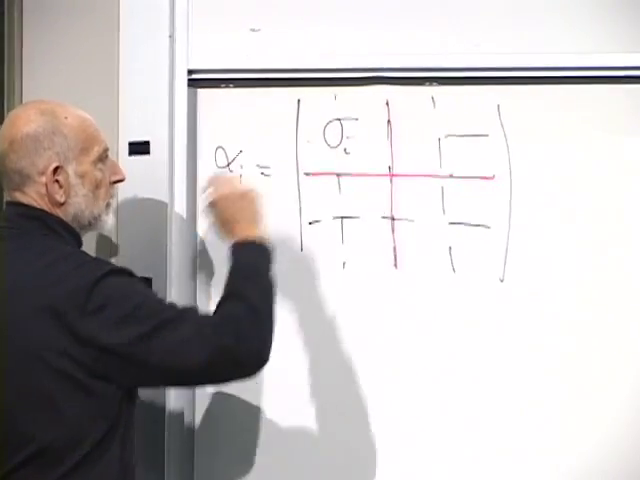
\includegraphics[width=0.68\textwidth]{lecture_08_figure_05.png}
\caption{Матрица Дирака \(\alpha_i\), записанная в виде блоков \(2\times2\), с \(\sigma_i\) и \(-\sigma_i\) на диагонали.}
\lectureframe{01:17:23}
\end{figure}

\begin{classroomqa}
\lecturetimestamp{01:17:41}
\audiencequestion{В более раннем представлении блоки \(\sigma_i\) были расположены наоборот?}
\lecturerresponse{Да. В другом представлении они стояли вне диагонали. Эти два расположения эквивалентны и связаны преобразованием подобия.}
\end{classroomqa}

В текущем представлении оставшаяся матрица имеет вид
\begin{equation}
\beta=
\begin{pmatrix}
0&I_2\\
I_2&0
\end{pmatrix},
\qquad
I_2=
\begin{pmatrix}
1&0\\
0&1
\end{pmatrix}.
\end{equation}
Поблочное умножение сводит проверку алгебры \(4\times4\) к обычному умножению матриц \(2\times2\).

\begin{classroomqa}
\lecturetimestamp{01:19:17}
\audiencequestion{Использовались ли в более раннем представлении другой знак или диагональная форма для \(\beta\)?}
\lecturerresponse{Там использовался другой, но физически эквивалентный базис. Замена базиса перемешивает четыре компоненты \(\Psi\) и меняет вид матриц, не изменяя физики.}
\end{classroomqa}

Четыре компоненты \(\Psi\) — это не четыре координаты пространства-времени. Это координаты в наименьшем векторном пространстве, на котором может действовать данная алгебра антикоммутации. Здесь есть две различные двукратные структуры: разбиение на блоки \(2\times2\) и двухкомпонентная структура Паули внутри каждого блока. Предвосхищая интерпретацию, установленную ниже, четыре возможности можно упорядочить так:
\begin{equation}
\begin{array}{c|cc}
& S_z=+\tfrac12 & S_z=-\tfrac12\\ \hline
\omega>0 & (\omega>0,+\tfrac12) & (\omega>0,-\tfrac12)\\
\omega<0 & (\omega<0,+\tfrac12) & (\omega<0,-\tfrac12)
\end{array}.
\end{equation}
Нижняя строка состоит из электронных состояний отрицательной частоты. Это не строка позитронов; позитрон будет интерпретирован как дырка в заполненном множестве этих состояний.

\section{Двукратная энергетическая структура в системе покоя и позитрон}

Двукратную энергетическую структуру легче всего выявить при нулевом импульсе. Когда \(\mathbf{k}=0\), состояние плоской волны пространственно постоянно, и член с пространственной производной исчезает. Уравнение в системе покоя\footnote{На кадре при \(01{:}23{:}38\) в массовом члене сохраняется временный лишний множитель \(i\); устное исправление при \(01{:}24{:}05\) устраняет его.} имеет вид
\begin{equation}
i\frac{\partial\Psi}{\partial t}=m\beta\Psi.
\end{equation}

\begin{figure}[t]
\centering
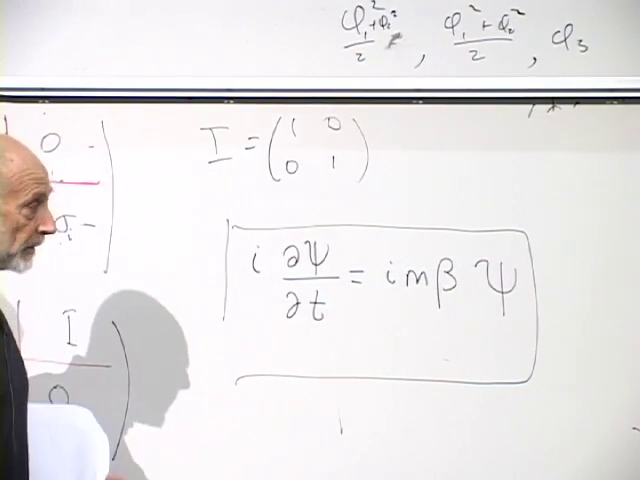
\includegraphics[width=0.76\textwidth]{lecture_08_figure_06.png}
\caption{При нулевом импульсе пространственные производные исчезают, и остается исправленное уравнение в системе покоя \(i\partial_t\Psi=m\beta\Psi\).}
\lectureframe{01:23:38}
\end{figure}

Разделим четырехкомпонентный столбец на верхний и нижний двухкомпонентные объекты:
\begin{equation}
\Psi=
\begin{pmatrix}
\psi_+\\
\psi_-
\end{pmatrix}.
\end{equation}

\begin{classroomqa}
\lecturetimestamp{01:24:47}
\audiencequestion{Означают ли обозначения \(\psi_+\) и \(\psi_-\) уже положительную и отрицательную энергию?}
\lecturerresponse{Нет. На этом этапе это лишь названия для верхнего и нижнего двухкомпонентных блоков. Их комбинации по энергии еще не найдены.}
\end{classroomqa}

\begin{classroomqa}
\lecturetimestamp{01:25:10}
\audiencequestion{Что представляет собой разделенный четырехкомпонентный столбец?}
\lecturerresponse{Это тот же самый четырехкомпонентный спинор Дирака, организованный так, чтобы соответствовать блочной форме матриц. Каждая половина является двухкомпонентным объектом, и две такие части образуют исходный четырехкомпонентный столбец.}
\end{classroomqa}

Матрица \(\beta\) меняет два блока местами:
\begin{equation}
\beta
\begin{pmatrix}
\psi_+\\
\psi_-
\end{pmatrix}
=
\begin{pmatrix}
\psi_-\\
\psi_+
\end{pmatrix}.
\end{equation}
Поэтому уравнение в системе покоя принимает вид
\begin{equation}
i\frac{\partial\psi_+}{\partial t}=m\psi_-,
\qquad
i\frac{\partial\psi_-}{\partial t}=m\psi_+.
\end{equation}

Есть две естественные возможности. Можно было бы взять еще одну производную по времени, чтобы развязать систему, но сложение и вычитание двух уравнений сразу их диагонализует. Действительно,
\begin{align}
i\frac{\partial}{\partial t}(\psi_++\psi_-)
&=m(\psi_++\psi_-),\\
i\frac{\partial}{\partial t}(\psi_+-\psi_-)
&=-m(\psi_+-\psi_-).
\end{align}
Введя
\begin{equation}
\chi_+=\psi_++\psi_-,
\qquad
\chi_-=\psi_+-\psi_-,
\end{equation}
получаем два независимых уравнения,
\begin{equation}
i\partial_t\chi_+=m\chi_+,
\qquad
i\partial_t\chi_-=-m\chi_-.
\end{equation}
При зависимости с определенной частотой \(e^{-i\omega t}\) для суммы имеем
\begin{equation}
\omega=+m,
\end{equation}
тогда как для разности имеем
\begin{equation}
\omega=-m.
\end{equation}
Это в точности то удвоение по положительной и отрицательной энергии, которое встретилось в более раннем одномерном примере: релятивистское уравнение вновь имеет электронные решения с положительной и отрицательной энергией. Тем самым блочное удвоение разделяется на ветви положительной и отрицательной энергии. Чистые состояния в системе покоя можно записать как
\begin{equation}
\Psi_{\omega=+m}=
\begin{pmatrix}
\xi\\
\xi
\end{pmatrix},
\qquad
\Psi_{\omega=-m}=
\begin{pmatrix}
\xi\\
-\xi
\end{pmatrix},
\end{equation}
где \(\xi\) по-прежнему является произвольным двухкомпонентным объектом.

Сумма и разность устранили одну двукратную структуру, но две компоненты \(\xi\) остаются. Матрицы Паули действуют на эту оставшуюся пару. Именно эта пара связана со спином и подлежит проверке на вращения и законы сохранения, обсуждаемой ниже.

\begin{classroomqa}
\lecturetimestamp{01:32:23}
\audiencequestion{Можно ли рассматривать спин как внешнюю двукратную структуру, а знак энергии — как внутреннюю?}
\lecturerresponse{Да. Эти два порядка факторов эквивалентны. Можно поменять, какой индекс писать первым; это всего лишь перестановка четырех компонент.}
\end{classroomqa}

Ветвь отрицательной частоты приводит к интерпретации моря Дирака. Отрицательной частоте приписывается отрицательная энергия электрона. Заполнение каждого электронного состояния с отрицательной энергией понижает энергию настолько, насколько это допускает принцип запрета, поскольку только один электрон может занимать каждое полное фермионное состояние. Тогда полностью заполненное море состояний с отрицательной энергией называется вакуумом.

Поднимем один электрон из этого заполненного моря в состояние с положительной энергией. В результате получаются электрон с положительной энергией и незанятое состояние с отрицательной энергией. Удаление отрицательной энергии повышает энергию, поэтому дырка имеет положительную энергию возбуждения; поскольку одного электрона недостаёт, она также несёт противоположный электрический заряд. Дырка — это позитрон.

\begin{classroomqa}
\lecturetimestamp{01:32:57}
\audiencequestion{Можно ещё раз пояснить интерпретацию позитрона?}
\lecturerresponse{Сумма двух блоков имеет положительную частоту, а разность — отрицательную. Решения с отрицательной частотой — это электронные состояния с отрицательной энергией, и вакуум получается при заполнении всех этих состояний. Если перевести один из занятых электронов на положительную энергию, остаются и электрон с положительной энергией, и дырка. Эта дырка с положительной энергией и противоположным зарядом и есть позитрон.}
\end{classroomqa}

Таким образом, алгебра сразу дала два следствия: ветви положительной и отрицательной энергии, которые дают структуру частица--античастица, и остающуюся двухкомпонентную структуру, связанную со спином 1/2. Примечательно, что обе возникли из наименьших матриц, способных удовлетворить релятивистским антикоммутационным соотношениям. К тому времени, когда эта математическая конструкция дала частицы со спином вместе с ветвью античастиц, спин лишь недавно вошёл в физику как эмпирически установленное свойство; в том историческом контексте результат был поразительным.

\begin{classroomqa}
\lecturetimestamp{01:35:14}
\audiencequestion{Являются ли сами электроны с отрицательной энергией позитронами?}
\lecturerresponse{Нет. Электронные состояния с отрицательной энергией заполнены в вакууме. Позитрон — это отсутствие одного электрона в этом заполненном наборе: дырка, а не электрон с отрицательной энергией.}
\end{classroomqa}

Дырка может участвовать в переходах. Позитрон имеет положительную энергию, потому что он представляет собой отсутствие электрона с отрицательной энергией. Если электрон с положительной энергией заполняет дырку, электрон и позитрон аннигилируют, но их энергия должна быть унесена, обычно фотонами. В терминах моря электрон заполнил незанятое состояние с отрицательной энергией. То же выделение энергии можно представить как переход возбуждённого электрона в атоме на более низкий уровень: при таком нисходящем переходе испускаются фотоны.

\begin{classroomqa}
\lecturetimestamp{01:36:39}
\audiencequestion{Почему более высоко лежащие электроны с отрицательной энергией не падают в дырку?}
\lecturerresponse{В этом вопросе смешиваются два случая. Заполнение дырки электроном с положительной энергией — это электрон--позитронная аннигиляция, при которой энергию уносят фотоны. Переход электрона из моря отрицательных энергий — это другой процесс, который рассматривается ниже.}
\end{classroomqa}

Сам по себе расчёт при нулевом импульсе установил двукратное вырождение после разделения по знаку энергии. Двукратное вырождение состояний само по себе не доказывает, что эти состояния несут угловой момент.

\begin{classroomqa}
\lecturetimestamp{01:37:44}
\audiencequestion{Каким образом расчёт при нулевом импульсе доказывает, что оставшаяся пара состояний соответствует спину?}
\lecturerresponse{Эту пару можно назвать состояниями вверх и вниз, и в полном уравнении появляются матрицы Паули, но само по себе это ещё не доказательство. Нужно показать либо как эта пара преобразуется при пространственных вращениях, либо что приписывание ей спина обеспечивает сохранение полного углового момента во взаимодействиях и столкновениях. Это доказательство откладывается.}
\end{classroomqa}

Для покоящегося состояния с положительной энергией верхний и нижний блоки равны,
\begin{equation}
\Psi_{\omega=+m}=
\begin{pmatrix}
\xi\\
\xi
\end{pmatrix}.
\end{equation}
Чтобы установить, что \(\xi\) является дублетом углового момента, требуется только что описанный аргумент, основанный на вращениях или на законе сохранения; это не следует просто из подсчёта двух компонент.

\begin{classroomqa}
\lecturetimestamp{01:40:46}
\audiencequestion{Может ли другой электрон аннигилировать с позитроном, даже если его энергия другая?}
\lecturerresponse{Да. Электроны не сохраняют индивидуальной идентичности. Любой доступный электрон может заполнить дырку, а различия в начальной энергии и импульсе отражаются в числе и энергиях испущенных фотонов.}
\end{classroomqa}

Картина с дырками объясняет также переход, целиком происходящий внутри моря отрицательных энергий. Предположим, занятое состояние с отрицательной энергией переходит в дырку. Исходная дырка заполняется, но состояние, из которого пришёл этот электрон, теперь пусто. Дырка переместилась. Эквивалентно можно сказать, что позитрон изменил свою энергию и испустил излучение.

\begin{classroomqa}
\lecturetimestamp{01:42:12}
\audiencequestion{Почему соседние уровни с отрицательной энергией не могут последовательно падать в дырку?}
\lecturerresponse{Могут: при этом дырка просто переходит с одного уровня на другой. Электрон, падая в прежнюю дырку, оставляет новую дырку на своей прежней энергии, так что исходный позитрон становится позитроном с другой энергией. Разность энергий уносится фотонами.}
\end{classroomqa}

\begin{classroomqa}
\lecturetimestamp{01:44:39}
\audiencequestion{Почему это не приводит к бесконечному нисходящему радиационному каскаду?}
\lecturerresponse{Потому что энергия и импульс должны сохраняться одновременно. Эти два закона сохранения не допускают неограниченного протекания такого процесса. Та же проблема возникает и для обычного свободного электрона: он не может просто продолжать понижать свою энергию, испуская фотоны в пустом пространстве.}
\end{classroomqa}